\chapter{Implementation}
\label{sec:implementation}
\INITIAL{T}{he proposed method} for implementing an in-situ visualization system is comprised of several vital parts. Although the  output visualization is key from a user perspective, there are important factors to be considered in the way that data is collected and how this method fits into the overarching analysis system. 
 
%%%%%%%%%%%%%%%%%%%%%%%%%%%%%%%%%%%%%%%%%%%%%%%%%%%%%%%%%%%%%%%%%%%%%%%%%%%%
%%%%%%%%%%%%%%%%%%%%%%%%%%%%%%%%%%%%%%%%%%%%%%%%%%%%%%%%%%%%%%%%%%%%%%%%%%%%
\section{Overview}
\label{sec:overview}
\INITIAL{T}{he core development portion of this work} is based on the classes which generate visualizations using a Flink execution plan. Firstly, there is an In-Situ Collector class which has the sole purpose of collecting data sets and/or summaries of data sets as they are run through the Flink analysis task. After data has been collected, the Visualizer can perform various visualization tasks based on the datasets which it has been provided. Figure \ref{fig:uml} shows the basic structural parts of this development. 

\paragraph{Visualization Classes}
While the aforementioned two classes perform the  bulk of the mechanical work, the visualizations themselves each require their own specialized classes which can be invoked generically from the Visualizer. For standard visualizations such as a histogram these classes largely handle the translation of data sets into a more easily digestible format which can be passed to pre-existing robust visualization libraries. In more complex and specific scenarios such as generating phrase nets, 'sketches' have been written in the Processing visualization language. These sketches can, with some minor modifications, be used within java projects and then drawn using the java swing toolkit. 

%%%%%%%%%%%%%%%%%%
\begin{figure}
	\centering
	\label{fig:uml}
	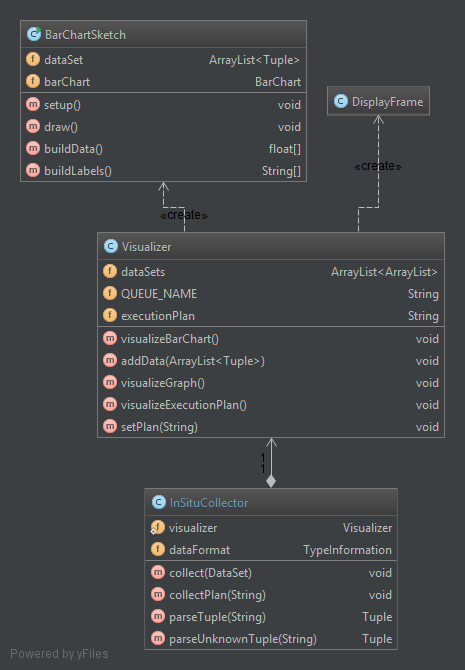
\includegraphics[scale=0.5]{uml_diagram.png}
	\caption{A UML diagram of the core classes}
	\TODO{Replace figure with updated/formatted version}
\end{figure}
%%%%%%%%%%%%%%%%%%

%%%%%%%%%%%%%%%%%%%%%%%%%%%%%%%%%%%%%%%%%%%%%%%%%%%%%%%%%%%%%%%%%%%%%%%%%%%%
%%%%%%%%%%%%%%%%%%%%%%%%%%%%%%%%%%%%%%%%%%%%%%%%%%%%%%%%%%%%%%%%%%%%%%%%%%%%
\section{Data Collection}
\label{sec:data_collection}
\INITIAL{D}{ata types in Flink} are analyzed by the optimizer to determine the most efficient execution strategies. In order to make this process simpler, Flink places limits on the types of data which can be used. There are four categories of types: General objects and POJOs, Tuples, Values, and Hadoop writeables. The handling of each of these types must of course be considered when data is being collected from an analysis graph.

\paragraph{Tuples}
Tuples are used to represent composite data sets, and are composed of a set length list of fields of various types. Tuples can include any valid Flink type as an element, including further tuples. One of the major benefits of using tuple types is the ability to use built-in functions to navigate through the tuple values. Specifically, these functions allow the selection of specific fields as the key for operations and more generally allow the navigation of tuple fields using string expressions.

\paragraph{Values}
Values are types which have their serialization and de-serialization specified manually.

\paragraph{Hadoop Writeables}
Objects which implement the Hadoop writeable interface.

\paragraph{Data Collector}
The data collector class acts as a simple addition to a pre-existing analysis program in Flink which collects data as it passes through operations. A single collector object exists for a given analysis flow, and collects data at a specific point with a single added line of code calling the collect method.

\paragraph{Collect Method}
Each time the collect method is called, it sends a new dataset to the central visualizer class. This method accepts a dataset as its sole argument and writes this dataset to memory in a format which can be read by the data collector. The data collector then reads this data into a new dataset outside of the original analysis flow's execution environment.
  
\paragraph{Data Sets}
A custom data set class exists for the use of the collector and visualizer. This class is very similar to the data set class which is native to Flink, but allows for the tracking of additional metadata which may be useful for debugging. This information could include timestamps, tags referring to specific operations in the analysis flow, or other semantically relevant information. These datasets are always initialized to contain tuple type objects. As a tuple can of course include any item of a basic type, this implementation will create a tuple of any general object in order to simplify data set operations. For example, if a single integer field is passed through the initial analysis flow, the data set generated in the visualizer will consider this as a tuple of size one which contains an integer.

\paragraph{Type Erasure}
When analysis jobs are executed, the java compiler will erase types and operate exclusively with generics. This means that when this data is extracted, some additional work is needed in order to determine a sufficient approximation of the original type for storage in a custom data set. To handle this, as each record is read into a data collector they are parsed through a set of pattern matching checks which determine the number of fields and the fields' types. Firstly, a simple line split determines the size of the tuples which should exist in the data set based on the input record. Next, each field is checked individually using the java string utilities library to determine whether they are numeric or non-numeric. Fields in each of these categories are then passed through a cascading set of conditional checks which determine their specific basic type, from least to most complex. For example, this method will attempt to parse a numeric field as an integer, and upon failure attempt to parse the field as a long. This process continues until a match is found; in the case that one is not an exception is thrown. 

%%%%%%%%%%%%%%%%%%%%%%%%%%%%%%%%%%%%%%%%%%%%%%%%%%%%%%%%%%%%%%%%%%%%%%%%%%%%
%%%%%%%%%%%%%%%%%%%%%%%%%%%%%%%%%%%%%%%%%%%%%%%%%%%%%%%%%%%%%%%%%%%%%%%%%%%%
\section{Distribution}
\label{sec:distribution}
\INITIAL{D}{istribution in analysis systems} following the general mapreduce model all operate very similarly in concept. This means that generally speaking, we can expect the dataset to be mapped into a set of key-value pairs which are then partitioned across a cluster in a uniformly distributed way. Because we may want to examine the intermediate dataset at a point prior to a reduce operation which would centralize the dataset, we must collect it piecemeal from each node in the cluster. This is achieved by sending the datasets from each node in the cluster to the visualizer for summary. 

\paragraph{Message Passing}
Message passing allows us to invoke a send message call from each in-situ data collector operating on a shard of the complete data set, and then receiving it in the visualizer. The visualizer can perform whichever operations are needed in order to merge the datasets considering the original locations and timing in order to generate useful output. 

\paragraph{Patterns?}
I'm not sure yet if a specific pattern will apply.

\paragraph{RabbitMQ}
So far arbitrary.

\paragraph{Specifics}
Implementation details such as server locale etc.

%%%%%%%%%%%%%%%%%%%%%%%%%%%%%%%%%%%%%%%%%%%%%%%%%%%%%%%%%%%%%%%%%%%%%%%%%%%%
%%%%%%%%%%%%%%%%%%%%%%%%%%%%%%%%%%%%%%%%%%%%%%%%%%%%%%%%%%%%%%%%%%%%%%%%%%%%
\section{Visualization}
\label{visualization}

\INITIAL{D}{eveloping visualizations} in software is a matter of both design and engineering. Finding an effective way to build visuals is often as important as selecting and conceptualizing the most appropriate way to convey the information at hand. In building the visualizations in this work, several languages and libraries have been applied in order to complete the work in the most effective way possible.

\paragraph{Processing}
Processing is a language which was initially developed as a teaching tool for computer programming fundamentals which utilized visual arts as a context. It was first released in 2001 as a project of the MIT aesthetics and computation group and has since evolved into a professional level tool for visual programming. The primary advantages of using Processing as a tool for the more complex portions of this work are it's ease of use, and compatibility with the rest of the development environment. As it was initially intended as a learning tool, the structure of a processing program is often very simple when compared with something similar generated using only java for example. A single program in Processing is referred to as a "sketch", referring to both the artistic nature of the language and the typical simplicity of it's application. In addition, processing code is compiled into java which simplifies the integration of the two. 

\paragraph{Libraries}
The City University of London's Graphical Information Center provides several useful libraries for performing visualization work. In particular, to aid in the development of work which utilizes processing sketches. The visualizations in this work have been built using classes from these utility libraries in the simplest of cases (such as the bar chart). In addition to providing basic visualizations in a pre-packaged format, there are some other tools such as navigational and formatting features which have been utilized in this work.  

\paragraph{Swing}
Outside of the visualizations themselves, the work of creating frames and navigation is largely handled through directly using java's swing visualization toolkit.

\paragraph{Presentation of Visualizations}
More comprehensive packaging, eventually.
